 %美赛模板:正文部分

\documentclass[12pt]{article}  % 官方要求字号不小于 12 号,此处选择 12 号字体
% \linespread{1.1}
% \bibliographystyle{plain}
% 本模板不需要填写年份,以当前电脑时间自动生成
% 请在以下的方括号中填写队伍控制号
\usepackage[2424527]{easymcm}  % 载入 EasyMCM 模板文件

\newcommand{\subsubsubsection}[1]{\paragraph{#1}\mbox{}\\}
\setcounter{secnumdepth}{4} % how many sectioning levels to assign numbers to
\setcounter{tocdepth}{4} % how many sectioning levels to show in ToC

\problem{B}  % 请在此处填写题号
% \usepackage{mathptmx}  % 这是 Times 字体,中规中矩 
\usepackage{palatino}  % mathpazo 这palatino是 COMAP 官方杂志采用的更好看的 Palatino 字体,可替代以上的 mathptmx 宏包
\usepackage{pdfpages}
\usepackage{longtable}
\usepackage{tabu}
\usepackage{threeparttable}
\usepackage{listings}
\usepackage{paralist}
\usepackage{multirow}
\usepackage{appendix}
\usepackage{siunitx}

\graphicspath{{img/}}          % 此处{img/}为相对路径,注意加上“/”
 \let\itemize\compactitem
 \let\enditemize\endcompactitem

\newcommand{\upcite}[1]{\textsuperscript{\textsuperscript{\cite{$\sharp$1}}}}
\title{Save the Submersible: Locate, Search, Rescue}  % 标题

% 如需要修改题头(默认为 MCM/ICM),请使用以下命令(此处修改为 MCM)
%\renewcommand{\contest}{MCM}

 %文档开始
\begin{document}

% 此处填写摘要内容
\begin{abstract}
    
 \indent On June 18, 2023, a deep-sea submersible lost contact while exploring the wreckage of the Titanic. After three days of search and rescue, it was confirmed that all five tourists were killed. This accident reminds us that as deep-sea exploration gradually moves into ordinary people's lives and becomes an optional entertainment project, the serious safety issues associated with the deep sea should also receive more attention. This article mainly explains the position prediction, search and rescue methods of the submersible after the accident and establishes the corresponding mathematical model, striving to provide complete safety measures.\\
 \indent In task 1, we built a predictive model of the submersible's position over time. Based on the information sent by the submersible to the main ship before the accident and real-time external data, combined with the knowledge of fluid mechanics, we calculate the acceleration of the submersible in all directions and use it as the observation value of Kalman filtering, using optimal estimation and state propagation and other methods to obtain the optimal solution and optimal distribution of real-time positions.\\
 \indent In task 2, we conduct a comprehensive evaluation of the main ship's search equipment, including laser detection devices, sonar, AUV (Autonomous Underwater Vehicle), and ROV (Remote Operated Vehicle), based on cost-effectiveness ratios. To measure effectiveness, we selected 3 main indicators, including range, precision, and accuracy, and determined their weights through the analytic hierarchy process. The results show that sonar has the highest overall score. In addition, in addition to search, it is best to equip the rescue ship with additional AUVs and ROVs for underwater rescue work.\\
 \indent In task 3, we established two models for specific search and rescue based on the positioning system. The random walk search model assumes that the direction and speed of the ocean current remain unchanged within a certain period of time. The search and rescue ship maintains a uniform motion with Gaussian noise in the direction of the ocean current, that is, the x-direction, and walks randomly in the y-direction. This model can conduct a large-scale search, but it is not suitable for situations where ocean currents change rapidly. The search success rate is about 68$\%$. The prediction following model uses the predicted position given by Kalman filter for real-time tracking, which is more efficient and accurate, with a success rate of about 90$\%$.\\
 \indent In task 4, for search and rescue problems in the Caribbean Sea, it is only necessary to read the position and speed of the ocean current where the submersible is located, and then the submersible's position can be found by relying on the aforementioned model;
 For the multi-submersible problem, the search method is the second search model in the third question, and the proximity principle tracking and judgment technology is added.\\
 \indent Additionally, we wrote a two-page reporting memo for the Greek government.

    % 美赛论文中无需注明关键字。若您一定要使用,
    % 请将以下两行的注释号 '%' 去除,以使其生效
    \vspace{5pt}  %mm	毫米	1 mm = 2.845 pt   pt 点	1 pt = 0.351 mm
    \textbf{Keywords}: Underwater Positioning; Kalman Filter; Gaussian Distribution; Cost-benefit Model; Optimal Position Estimation

\end{abstract}

\maketitle  % 生成 Summary Sheet

\tableofcontents  % 生成目录


% 正文开始
% Chapter 1: Introduction
\section{Introduction}

\subsection{Problem Background}
The existing underwater positioning technology basically originates from imitating the positioning mode of underwater creatures, that is, bionics. In the course of a century of development,
the efficiency and accuracy of underwater positioning have been continuously improved.
But this is all based on the close cooperation between the host ship and underwater detection equipment. However, emergencies happen from time to time, such as On 18 June 2023, Titan, a submersible operated by American tourism and expeditions company OceanGate, imploded during an expedition to view the wreck of the Titanic in the North Atlantic Ocean off the coast of Newfoundland, Canada . 
Therefore, we must be prepared for possible emergencies, such as the loss of contact with a submersible. Using known information to build a model of a submersible's location can help predict a submersible's location if contact with the submersible is lost. This technology is based on the fact that the host ship has certain detection equipment, such as radar and sonar, and can receive ocean data through satellites. In this problem, we will also model the location of the lost submersible in this context and consider the issue of maximum efficiency of search and rescue equipment.
In addition, we will also measure the optimal initial position of the search and rescue equipment and make reasonable extrapolations.
\begin{figure}[htbp]  %h此处,t页顶,b页底,p独立一页,浮动体出现的位置
\centering  %图表居中
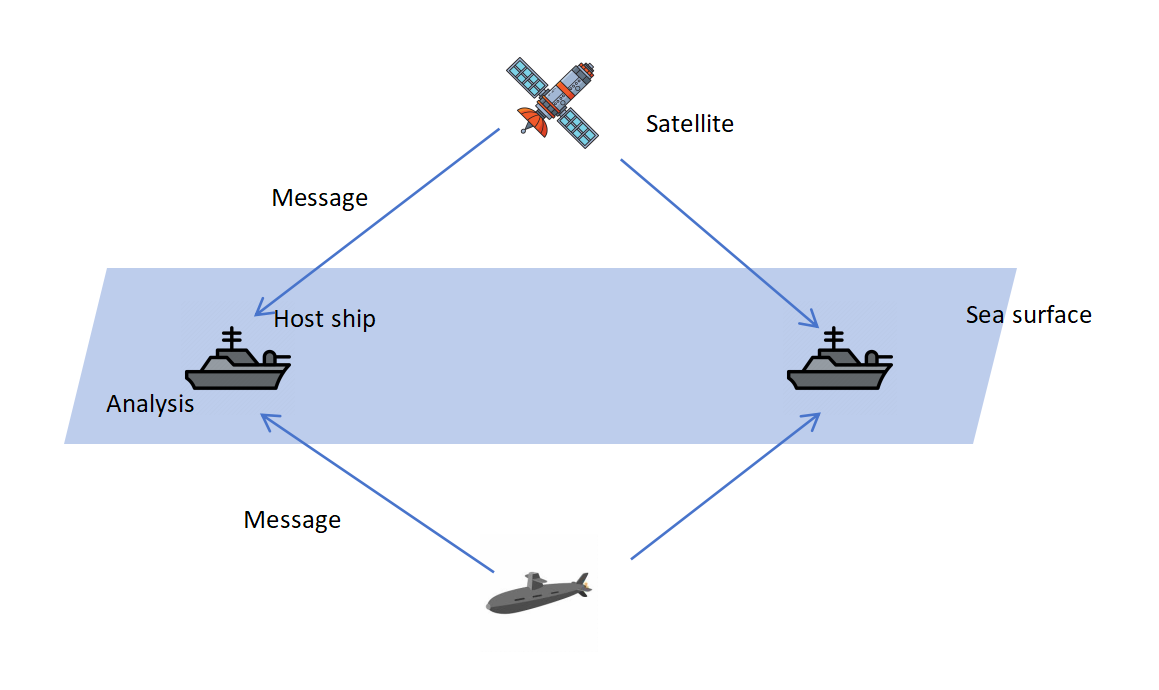
\includegraphics[width=.7\textwidth]{background.png} %图片的名称或者路径之中有空格会出问题 
\caption{Underwater positioning diagram} % 图片标题 

\end{figure}
\subsection{Restatement of the Problem}
Our main goal is to use known information to locate the missing submersible while solving search related problems.
For this, we need to solve the following problems:

\begin{itemize}
\setlength{\parsep}{0ex} %段落间距
\setlength{\topsep}{2ex} %列表到上下文的垂直距离
\setlength{\itemsep}{1ex} %条目间距
\item Establish a mathematical model to speculate on the location of the missing submersible and calculate the uncertainty.
\item For the search problem, a cost-benefit model is established to consider costs and efficiency.
\item Based on the positioning model, establish a model of the probability of finding the submersible, and determine the initial position of the search and rescue equipment;
\item Apply the model to practice, explore positioning models in different sea areas, and consider the presence of multiple submersibles.
\end{itemize}

\subsection{Our Work}
The problem requires us to fight fires by optimizing the locations of two type of drones. Our work mainly includes the following:
\begin{enumerate}[\bfseries 1.]
    \setlength{\parsep}{0ex} %段落间距
    \setlength{\topsep}{0.5pt} %列表到上下文 的垂直距离
    \setlength{\itemsep}{0.5pt} %条目间距
    \item Use Kalman filter to fuse submersible acceleration observation data and historical data to obtain the optimal solution and optimal distribution of real-time position;
    \item The cost-benefit ratio is used to evaluate the comprehensive evaluation score of the search equipment to select the most suitable equipment, where the benefits are calculated using the analytic hierarchy process;
 \item Based on the positioning model, establish a model of the probability of finding the submersible, and determine the initial position of the search and rescue equipment;
    \item Apply the model to practice, explore positioning models in different sea areas, and consider the presence of multiple submersibles.
\end{enumerate}  %三和四都得改% 
In order to avoid complicated description, intuitively reflect our work process, the flow chart is shown in Figure 2:

\begin{figure}[htbp]  %h此处,t页顶,b页底,p独立一页,浮动体出现的位置
\centering  %图表居中
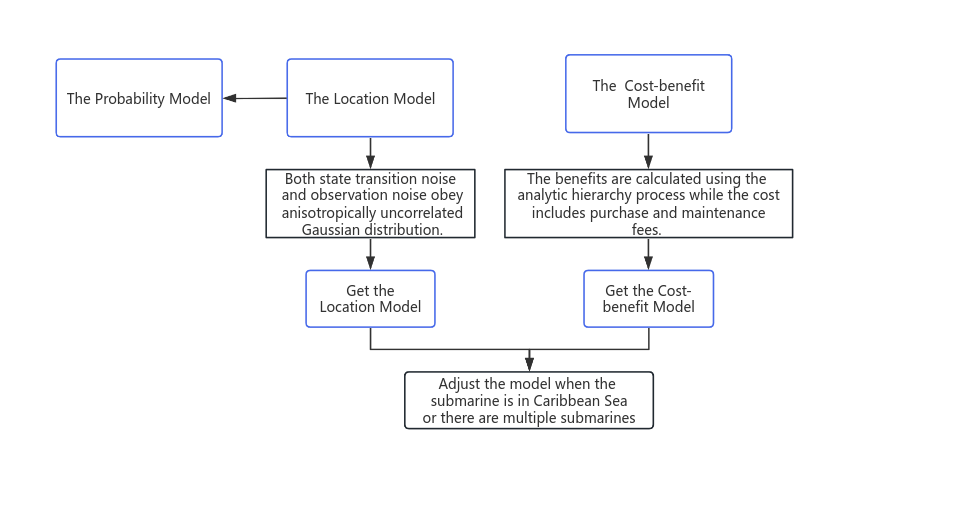
\includegraphics[width=.9\textwidth]{ourwork.png} %图片的名称或者路径之中有空格会出问题 
\caption{Flow Chart of Our Work} % 图片标题 
\end{figure}
\vspace{-0.8cm}

\section{Assumptions and Explanations}
Considering that practical problems always contain many complex factors, first of all, we need to make reasonable assumptions to simplify the model, and each hypothesis is closely followed by its corresponding explanation:

\begin{enumerate}[\bfseries \textit{Assumption} 1:]
	\item \textbf{Both state transition noise and observation noise obey anisotropically uncorrelated Gaussian distribution.}\\
	\textbf{\textit{Explanation:}}The uncertainty of the indirect acceleration measurement instrument is the same in three directions and is independent in all directions.
	\item \textbf{Average annual failure rate and usage costs can be ignored in the calculation.}\\
	\textbf{\textit{Explanation:}}Compared with the purchase cost, the annual average failure rate and usage cost account for a small proportion and will not have a significant impact on the cost-benefit calculation model.
	\item \textbf{The shape of the submersible is considered to be spherical.}\\
	\textbf{\textit{Explanation:}}Since it is on the seabed, the impact of the submersible's size and shape is negligible. Equivalent to a spherical submersible, the calculation can be simplified and the influencing factors in modeling can be reduced.
	
\end{enumerate}
Additional assumptions are made to simplify analysis for individual sections. These assumptions will be discussed at the appropriate locations.

\section{Notations} %记号
Some important mathematical notations used in this paper are listed in Table 1. 
\begin{table}[htbp]
\begin{center}
\caption{Notations used in this paper}
\begin{tabular}{c l}
\toprule[2pt]
\multicolumn{1}{m{3cm}}{\centering Symbol}
&\multicolumn{1}{m{8cm}}{\centering Description }\\
\midrule
$CER$& Cost Effect Ratio \\
$C$& Cost \\
$E$& Effect \\
$P$& Precision \\
$A$& Accuracy \\
$R$& Range \\
$\omega$& Weight\\
$x_k$ & $k^{th}$ true state\\
$x^-_k$ & $k^{th}$ state prediction \\
\vspace{5pt}%公式间有点挤,空一些
$\hat{\mathbf{x}_k}$ & $k^{th}$ optimized state estimation\\
\vspace{3pt}
$e^-_k$ & prediction error = $x^-_k-x_k$\\
$\hat{\mathbf{e}_k}$ & estimation error = $\hat{\mathbf{x}_k}-x_k$\\
F & state transition Matrix\\
G & control-state Matrix\\
H & Observation Matrix\\
$w_k$ & state noise, $w_k$\textasciitilde N[0,$Q_k$)\\
$v_k$ & observation noise, $v_k$\textasciitilde N[0,$R_k$)\\

\bottomrule[2pt]
\end{tabular}\label{tb:notation}
 \begin{tablenotes}
        \footnotesize
        \item[*] *There are some variables that are not listed here and will be discussed in detail in each section. %此处加入注释*信息
      \end{tablenotes}
\end{center}
\end{table}
\vspace{-1cm}%在\end{table}下加一行\vspace{-1cm} 其中-1的作用是缩短与下方文字距离的 切记!必须是负数

\section{Model Preparation}
\subsection{Data Overview}
The question did not provide us with data directly, so we need to consider which data to collect in the model building. 
Through the analysis of the problem, we need to collect the relevant information of
densities in the sea,the geography of the
sea floor, the type of search
equipment and costs associated with availability, maintenance,
readiness, and usage of this equipment and so on. 
Due to the large amount of data, it is not convenient to list them all, the data not listed will be discussed in detail in each section.

\subsubsection{Data Collection}
Data sources are shown in Table 2.

\begin{table}[htbp]
\begin{center}
\caption{Data and Database Websites}
\resizebox{\textwidth}{!}
{\begin{tabular}{c c}
\toprule[2pt]
\multicolumn{1}{m{5cm}}{\centering \textbf{Database Names}}
&\multicolumn{1}{m{10cm}}{\centering \textbf{Database Websites} }\\ %m后面是列宽
\midrule
Oceanography Big Data& https://www.casodc.com/search-field \\
GMRT Map Tool & https://www.gmrt.org/GMRTMapTool/ \\
Chasing ROV & https://www.chasing.com/zh\\ 
Google Scholar & https://scholar.google.com/ \\
Maps& \copyright{} 2021 Mapbox \copyright{} OpenStreetMap\\
\bottomrule[2pt]
\end{tabular}}
\end{center}
\end{table}

\section{Positioning system based on Kalman filter}%第一个模型
\subsection{Physics model}

\subsubsection{Vertical Direction}
\begin{equation}
    \begin{aligned}
     \mathbf{T}=T_0-A*e^{-bh}
\end{aligned}
\end{equation}
\indent Notations: T: The temperature of the ocean; A,b: Const; h: Depth; 
$T_0$: The temperature of the ocean when h=0.\\

\begin{equation}
    \begin{aligned}
     \mathbf{\rho}=\rho_0+a*(s-s_0)+\beta*(T-T_0)
\end{aligned}
\end{equation}

\indent Notations: $\rho_0$: Reference density; $S_0$: Reference salinity; $T_0$: Reference temperature; \\

\indent Salinity changes with depth

\begin{equation}
    \begin{aligned}
     \mathbf{s}=s_0-k*h
\end{aligned}
\end{equation}

\indent Notations: k: Coefficient of variation\\

Substitute equation (1) and (3) into equation (2) to get:
\begin{equation}
    \begin{aligned}
        \mathbf{\rho(h)}=\rho_0+k_1*h+k_2*e^{-k_3*h}
\end{aligned}
\end{equation}

\begin{equation}
    \begin{aligned}
        \mathbf{k_1}=k*\alpha
\end{aligned}
\end{equation}

\begin{equation}
    \begin{aligned}
\mathbf{k_2}=A*\beta
\end{aligned}
\end{equation}

\begin{equation}
    \begin{aligned}
\mathbf{k_3}=b
\end{aligned}
\end{equation}

\begin{equation}
    \begin{aligned}
\mathbf{F_{float}}=\rho*g*h
\end{aligned}
\end{equation}

\indent Therefore, at vertical direction
\begin{equation}
    \begin{aligned}
\mathbf{F_{float}}=m*g+m*a_2
\end{aligned}
\end{equation}

\subsubsection{Horizontal Direction}
\indent First simplify the submarine into a capsule model\\
\indent Definition: Strokes: F=f(H/ $R_e$)=0.700*$\left(H/ R_e\right)^{-1.082}$+1.001\\
\indent Notations: y: Dynamic viscosity; u: The undisturbed fluid velocity at the center line 
of the space; $R_E$: Equivalent sphere radius\\
\indent $F_x$=m*$a_x$ $F_y$=m*$a_y$ \\
\indent Due to modeling needs, the submarine is equivalent to a sphere in the following explanation. Therefore, the equivalent radius in the above formula is the spherical radius.

\subsection{Kinematics model}
\indent The acceleration obtained from the observation data has unpredictable observation noise and is consistent with the random walk model. 
Direct kinematic solution without modeling and estimating the noise can easily cause the cumulative error to affect the prediction and thus the position estimation result. Therefore, The Kalman Filter method is used here to fuse observation data and state data to find the optimal posterior distribution and improve the confidence of the prediction results.

\subsubsection{State definition}
\indent State Vector
\begin{equation} 
    \begin{aligned}
  \mathbf{x}=
  \begin{bmatrix}
    p^T_{3*1}&v^T_{3*1}&a^T_{3*1}
  \end{bmatrix}
\end{aligned}
\end{equation}


\begin{equation}
    \begin{aligned}
x_k=F_k*x_{k-1}+G_k*u_k+w_k
\end{aligned}
\end{equation}

\indent    G = Any, if given $u_k$ = 0\\
\indent   R, Q is fixed.

\indent State Transition Matrix
\begin{equation}
    \begin{aligned}
F = \begin{bmatrix}
    1&0&0&\Delta t&0&0&0&0&0
    \\0&1&0&0&\Delta t&0&0&0&0
    \\0&0&1&0&0&\Delta t&0&0&0
    \\0&0&0&1&0&0&\Delta t&0&0
    \\0&0&0&0&1&0&0&\Delta t&0
    \\0&0&0&0&0&1&0&0&\Delta t
    \\0&0&0&0&0&0&1&0&0
    \\0&0&0&0&0&0&0&1&0
    \\0&0&0&0&0&0&0&0&1
    \end{bmatrix}_{9*9}
\end{aligned}
\end{equation}

\indent Observation Equation

\begin{equation}
    \begin{aligned}
z_k=H_k*x_k+v_k
\end{aligned}
\end{equation}

\indent 

\subsubsection{State Propagation}
\begin{equation}
    \begin{aligned}
x_k=F_k*x_{k-1}+G_k*u_k
\end{aligned}
\end{equation}
\begin{equation}
    \begin{aligned}
        P^-_k=F_k*P_{k-1}*F^T_k+Q
    \end{aligned}
\end{equation}

\subsubsection{State Update}

\begin{equation}
    \begin{aligned}
        \hat{\mathbf{x}_k}=x^-_k+K_k(Z_k-H_k*x^-_k)
    \end{aligned}
\end{equation}

\begin{equation}
    \begin{aligned}
        P_k=(I-K_k*H_k)P^-_k
    \end{aligned}
\end{equation}

\begin{equation}
    \begin{aligned}
        K_k=P^-_k*H^T(H*P^-_k*H^T+R)^{-1}
    \end{aligned}
\end{equation}

\begin{figure}[htbp]  %h此处,t页顶,b页底,p独立一页,浮动体出现的位置
    \centering  %图表居中
    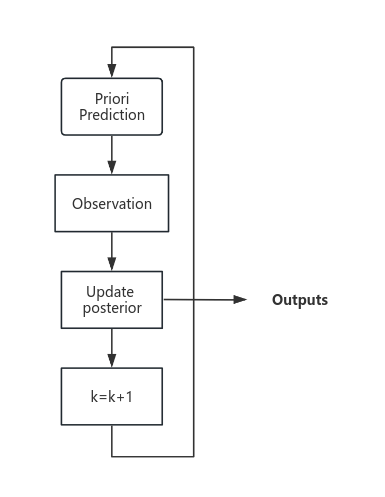
\includegraphics[width=.6\textwidth]{model1.1.png} %图片的名称或者路径之中有空格会出问题 
    \caption{Flow Chart of Model 1} % 图片标题 
    \end{figure}
    \vspace{-0.8cm}

\subsection{Conclusion}\
\indent Using known information and fluid mechanics knowledge, the acceleration in the three directions of XYZ is solved through ocean current calculation. In the Kalman filter, they are used as observations, and the above equations, optimal estimation, state propagation, etc. are used, combined with the current state data, to obtain the optimal solution for the current position estimate. At the same time, this is used as the posterior distribution in the third question to give the optimal delivery point.

\section{Economic benefit model for additional search equipment}
\indent At present, there are a wide variety of underwater detection and search equipment worldwide. Through analysis of the problem, based on literature and surveys, we classify the relevant search equipment that can be equipped on the host ship into four categories: laser detection system, sonar, ROV and AUV, which further comprehensive consideration and analysis is based on. (Note: The first two refer to direct installation on the host ship for search, while the latter two are submerged for exploration. In fact, it’s often the case that the latter two also include laser radar and sonar as a part of their structure to achieve search functions.)
The selection of search equipment should be based on a comprehensive consideration of practicality and economy, namely cost and effect. To be exact, cost includes the related expenses for purchase, maintenance, and use. As for the effect, we refined 16 evaluation indicators through 8 relevant theses, and ultimately retained the three most meaningful indicators in the discussion of this issue, including detection range, accuracy, and precision.
Since the Ionian Sea in the scenario is a branch of the Mediterranean Sea with an average depth of about 1,450 meters and a maximum depth of 5,121 meters, and the submersible is intended to be used to take tourists on an undersea adventure in this sea area, we believe that a search device with a detection depth of at least 500 meters should be selected for procurement. Based on this, we extensively collected data from various search devices, excluded some abnormal values, and took the median as the data for this type of search equipment.
\subsection{Cost Effect Ratio}
\indent We use the cost-effectiveness ratio (hereinafter referred to as CER) to measure the comprehensive performance of the search equipment to find the most suitable type.
\begin{equation}
    \begin{aligned}
     CER =  {E/C} 
     \end{aligned}
    \end{equation}
\subsection{Cost}
\indent C= Purchase Price/Service Life + Annual Maintenance Cost + use cost * annual average failure rate of the submersible (+ personnel training cost)
\subsection{Effect}
When calculating the effect, due to the different importance of detection range, accuracy, and precision in practical applications, we need to first calculate the weights corresponding to the three indicators, and then obtain E through the following formula:
\begin{equation}
    \begin{aligned}
E=\omega_1*P+\omega_2*A+\omega_3*R
 \end{aligned}
      \end{equation}
Through analysis, we can found that all three are positive indicators.
\subsubsection{Data Normalization}
\indent In order to eliminate the influence of different dimensions on calculations, we need to normalize data with different units to facilitate further calculations at the same scale.
Since the above indicators are all positive indicators, that is, "benefit attributes type", the following formula is used for positive normalization:
\begin{equation}
    \begin{aligned}
        \widetilde{x_{ij}} =  \frac{x_{ij}-min\{x_{ij}\}}{max\{x_{ij}\}-min\{x_{ij}\}}
     \end{aligned}
    \end{equation}
\indent  Suppose there are m sets of data in each of the accuracy (i=1), precision (i=2), and range (i=3) dimensions, where $x_{ij}$ represents the $j_{th}$ data in the $i_{th}$ set, max{$x_i$} represents the largest data in the i-th set, and min{$x_i$} represents the smallest data in the $i_{th}$ set.

\subsubsection{AHP (analytic hierarchy process)}
\indent The analytic hierarchy process (AHP) refers to a systematic method for optimizing decision-making in a complex, multi-objective setting by considering the problem as a system, decomposing the objectives into multiple objectives or criteria, and further decomposing them into multiple levels of indicators (or criteria, constraints). Through a qualitative and fuzzy quantitative approach, the single ranking (weight) and overall ranking of the levels are calculated to serve as the objective (multi-indicator) and multi-proposal optimization decision-making system.
 \subsubsubsection{Construct the judgement matrix}
 \indent In order to calculate the weights of these three indicators and obtain the utility score of this type of search equipment, based on the analysis of the question, we ranked the importance of these three indicators in the selection of search equipment as follows: range > accuracy > precision. Based on this judgement, we construct the judgement matrix.
 \begin{equation}
    \begin{aligned}
        \widetilde{x_{ij}} =  \frac{x_{ij}-min\{x_{ij}\}}{max\{x_{ij}\}-min\{x_{ij}\}}
     \end{aligned}
    \end{equation}

    \subsubsubsection{Calculate the weights of each indicator}
    \indent The arithmetic mean, geometric mean, and eigenvalue methods are used to obtain the relative weights of each indicator. The decision matrix is used as the basis for weight calculation.

    \begin{table}[H]
        \centering
        \caption*{\textbf{Table:} AHP results}
        \begin{tabular}{|c|c|c|c|c|c|c|c|}
            \hline
            \textbf{Item}  & \textbf{Eigenvector} & \textbf{Weight (\%)} & \textbf{maximum characteristic root} & \textbf{CI}  \\ \hline
            \textbf{precision}  & 0.131   & 4.37    & \multirow{3}{*}{3.004 }     & \multirow{3}{*}{0.002  }          \\ 
            \textbf{accuracy}  &1.391   & 46.366    &  \multirow{3}{*}{}    &  \multirow{3}{*}{}           \\ 
            \textbf{range}  & 1.478   & 49.264    &  \multirow{3}{*}{ }      &  \multirow{3}{*}{}          \\ \hline
        \end{tabular}
    \end{table}
  \indent $\omega_1$=0.0437  $\omega_2$=0.46366  $\omega_3$=0.49264

  \subsubsubsection{Consistency test}
  \begin{equation}
    \begin{aligned}
     CR =  {CI/RI} =0.04
     \end{aligned}
    \end{equation}
  \indent This consistency is acceptable.

  \subsubsection{Results and Analysis}
  \indent Substituting the above weights into the calculation, we obtain:

  \begin{table}[H]
    \centering
    \caption*{\textbf{Table:} Original$\_$Data$\_$1}
    \begin{tabular}{|c|c|c|c|c|c|c|c|}
        \hline
        \textbf{type}  & \textbf{Effect} & \textbf{CER}  \\ \hline
        \textbf{Laser detection}  & 0    & 0    \\ \hline
        \textbf{Sonar}  & 0.633062242 &12.6108 \\ \hline
        \textbf{AUV}  & 1& 1.234568  \\ \hline
        \textbf{ROV}  & 0.82714386    & 0.818954           \\ \hline
    \end{tabular}
\end{table}

\indent Comprehensive analysis shows that the most cost-effective is sonar, while the lowest score is given to lidar mainly due to its low depth detection.
AUV and ROV generally don’t have a relatively high score in cost-benefit analysis of search equipment, but in actual rescue operations, as the sonar is only able to search and locate the submersibles, AUV and ROV should be equipped on the rescue ship for the recovery and rescue of submersibles.

\section{Determine Initial Position of the equipment and the Probability}%第三个模型

The conditions for the activation of search and rescue equipment are that the submersible is one kilometer away from the search and rescue equipment and the submersible is lost.\\
\indent Combined with search and rescue equipment, as long as there is a target ship within the search radius, it is considered to have been searched and can be judged to be successful.\\
\indent On the contrary, as long as the number of searches exceeds a certain threshold, it will be judged as failed, because at this time the Kalman filter already has a large cumulative error, and the credibility of the results is extremely low, making search and rescue impossible.\\
\indent P.S. After monitoring, $v_1$=$v_2$ finally stabilized at $seaspeed_x$.



\subsection{Random-walk Search Model}
\indent Assume that the direction and speed of the ocean current remain unchanged for a period of time. Set the ocean current direction as x and the vertical direction as y. The search and rescue ship maintains uniform motion with Gaussian noise in the x direction and walks randomly in the y direction.As the picture shows:

\begin{figure}[htbp]  %h此处,t页顶,b页底,p独立一页,浮动体出现的位置
    \centering  %图表居中
    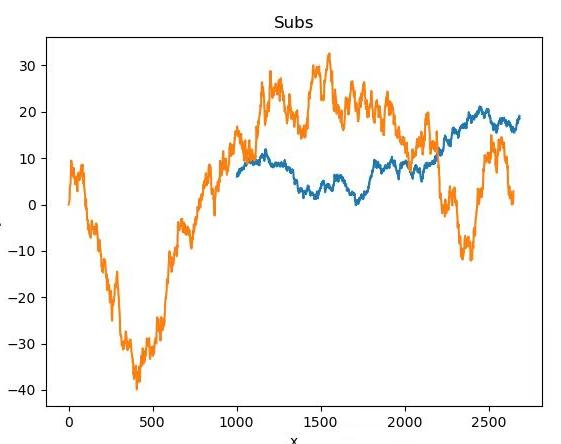
\includegraphics[width=.9\textwidth]{randomwalk111.jpg} %图片的名称或者路径之中有空格会出问题 
    \caption{Experimental results} % 图片标题 
    \end{figure}
    \vspace{-0.8cm}
    \indent \\

\indent The orange curve represents the simulated position of the search ship in the first algorithm;\\
\indent The blue curve represents the swimming position of the submersible.
    \subsubsection{Model overview}
    $\sharp$  model: submersible\\
     $\sharp$ $x$ = $x$ + $v_x$dt\\
    $\sharp$ $y$ = $y$ + $v_y$dt\\
    $\sharp$ $v_x$ = $v_x$ +  $x_{random}$\\
    $\sharp$ $v_y$ = 0 +  $y_{random}$\\
    $\sharp$ Supposed that in a small area, the flow goes mainly one way.\\
    
    $\sharp$ model: search boat \\
    $\sharp$ $x$ = $x$ + $v_x$dt\\
    $\sharp$ $y$= $y$ + $v_y$dt\\
    $\sharp$ $v_x$ = $v_x$$\pm$0.5\\
    $\sharp$ $v_y$ = 0 + $y_{random}$\\
    $\sharp$ Suppose that flows has no effect on search boat.\\


    \subsubsection{Model Analysis}
    \indent Advantages: It can conduct a wide range of searches and does not require high positioning accuracy. It is possible to search and rescue even if the cumulative error is too large.\\

    Shortcomings: The search success rate is too low, around 0.68, and is not suitable for situations where ocean currents change quickly, abruptly, and in large directions.

    \subsection{Prediction Following Model}
\indent Using the predicted position given by the Kalman filter, the ship's bow always moves forward in the direction of the real-time predicted position. By giving the real-time position, real-time tracking adjustment is achieved, and the ship approaches the predicted point at the fastest theoretical speed, which greatly improves efficiency. . As for why we don’t consider running directly to the predicted intersection position, that’s because the Kalman filter gives real-time information. When future observations are uncertain, predicting distant future positions will produce huge cumulative errors.

\subsubsection{Model overview}

\indent $\sharp$ $v_{x2}$ = searchspeed * $\left(x_{e1} - x_2\right)$ / $\sqrt{\left( \left(x_{e1} - x_2\right)^{2} + \left(y_{e1} - y_2\right)^{2}\right)}$\\
\indent $\sharp$ $v_{y2}$= searchspeed *$\left(y_{e1} - y_2\right)$ / $\sqrt{\left( \left(x_{e1} - x_2\right)^{2} + \left(y_{e1} - y_2\right)^{2}\right)}$\\
\indent $\sharp$ $x_2$ = $x_2$ + $v_{x2}$*dt\\
\indent $\sharp$ $y_2$ = $y_2$ + $v_{y2}$*dt\\

\indent $x_{e1}$, $y_{e1}$ refers to the Kalman filter's estimate of $x_1$, $y_1$, which will produce cumulative errors. The submersible's motion model is the same as the one set up in the first model.

\subsubsection{Model Experiment}
\indent The blue curve represents the submersible position;\\
\indent The orange curve represents the predicted position;\\
\indent The green curve represents the search device position.\\   
\indent In this model, the probability of finding the submersible is nearly 0.9\\
(In five rounds, the results are 0.907 0.917 0.907 0.898 0.918). 
\begin{figure}[htbp]  %h此处,t页顶,b页底,p独立一页,浮动体出现的位置
    \centering  %图表居中
    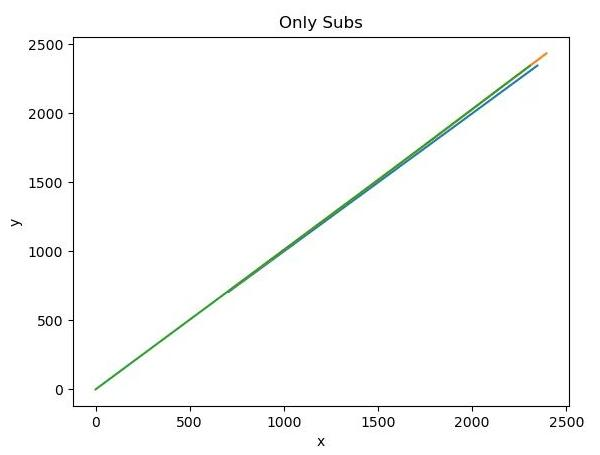
\includegraphics[width=.7\textwidth]{predictionfollowing.jpg} %图片的名称或者路径之中有空格会出问题 
    \caption{Experimental results} % 图片标题 
    \end{figure}
    \vspace{-0.8cm}

\indent \\
\indent \\
\indent \\
\indent \\
\indent \\
\indent \\
\indent \\
\indent \\
\indent \\

\subsubsection{Model Analysis}
\indent Advantages:Since the prediction quantity is the optimal estimate of the posterior variance, the probability of search success can be maximized. At the same time, the bow of the ship is always aligned in the predicted direction, which can save fuel to the maximum extent and ensure the efficiency of search and rescue. When the cumulative error does not reach a large value in a short period of time, a very accurate estimate can be provided.\\
\indent Shortcomings:The performance is too strong in a short period of time and the long-term drift cannot be estimated, which may cause the prediction results to deviate from the true position of the submersible; When encountering extreme situations (for example, when a submersible enters a small underwater vortex, or when the submersible's state quantity or observation quantity in a certain direction is always hovering near 0), large mutations will occur, resulting in inaccurate positioning and performance problems. Not as good as the first model, but it is suitable for most situations (the experiment simulated the predicted tracking situation of the ocean currents becoming faster and slower, and changing direction).


\subsection{Probability Model}
Fitting Function:\\
\indent Definition: sigmoid(t,a,b,c) a=2.37704058 b=165-1.05018821 c=0.9117708 t: time\\
\indent Return: c/(1+$e^{-a*\left(t-b\right)}$)\\
\indent Notations:

\begin{equation}
    \begin{aligned}
     t=array[1,2,3,4,5]
     \end{aligned}
    \end{equation}
    \begin{equation}
        \begin{aligned}
         y=array[0.1,0.4,0.5,0.9,1.0]
         \end{aligned}
        \end{equation}
      \indent  Fitting method: Least Squares Method

        \begin{figure}[htbp]  %h此处,t页顶,b页底,p独立一页,浮动体出现的位置
            \centering  %图表居中
            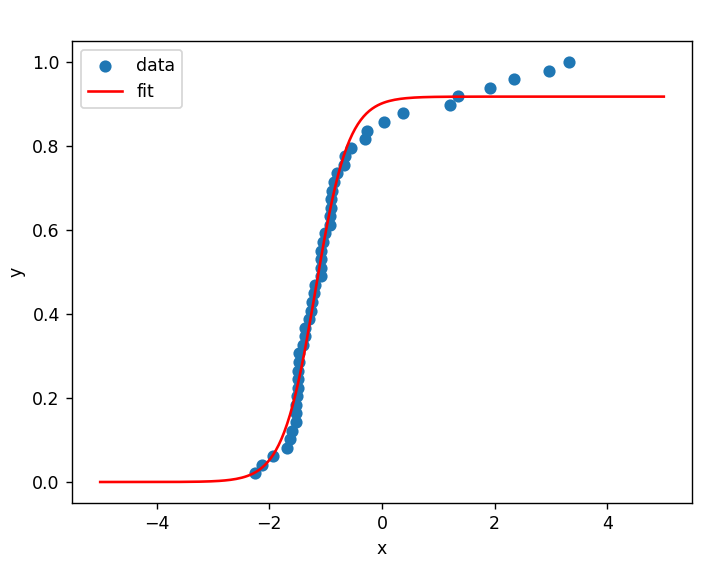
\includegraphics[width=.7\textwidth]{probability.png} %图片的名称或者路径之中有空格会出问题 
            \caption{Experimental results} % 图片标题 
            \end{figure}
            \vspace{-0.8cm}
    \indent \\
           \indent Correlation factor: $R^{2}$=0.922\\
\indent It can be seen from the experimental results that this model has good efficiency.

    \section{Caribbean Sea and Multiple Submersible} %第四个模型
\subsection{The Caribbean Sea}
    \indent By importing the speed of ocean currents and the salinity of seawater in the Caribbean Sea, and adjusting the parameters in the first model, the positioning model of the Caribbean Sea is obtained.\\
\indent The hydrological properties of the Caribbean Sea are highly homogeneous. Taking the monthly average temperature of the sea surface as an example, the annual variation does not exceed 3$^{\circ}$C (25$^{\circ}$C-28$^{\circ}$C). The Caribbean Sea has a salinity of 3.6$\%$ and a density of 1.0235-1.0240*$10^{3}$kg/m3. The main current in this sea area is the Caribbean Current, a warm current formed by the convergence of part of the North Equatorial Warm Current of the Atlantic Ocean and the Guyana Current into the Caribbean Sea. The average flow velocity is 38 to 43 cm/second.\\
\indent What's more, according to the Physics model established in the first model:\\
\indent  $\rho(h)$=$\rho_0$+$k_1$*h+$k_2$*$e^{-k_3*h}$\\
\indent At vertical direction $F_{float}$=m*g+m*$a_2$\\
\indent Only by bringing the seawater density and ocean depth of the Caribbean Sea into $\rho(h)$ and h in the equation respectively, the positioning model of the Caribbean Sea can be established.


\subsection{Multiple Submersible}
\indent Use the proximity principle to determine the submersible closest to the search and rescue equipment. And every time the bow is adjusted, the position of the nearest submersible is re-determined, and the best search position is finally found.\\
\begin{figure}[htbp]  %h此处,t页顶,b页底,p独立一页,浮动体出现的位置
    \centering  %图表居中
    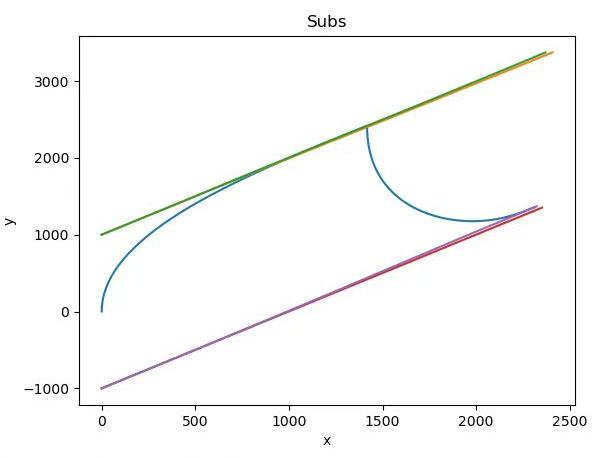
\includegraphics[width=.7\textwidth]{mul.jpg} %图片的名称或者路径之中有空格会出问题 
    \caption{Experimental results} % 图片标题 
    \end{figure}
    \vspace{-0.8cm}
    \indent \\
\indent Green curve - predicted position of submarine 1\\
\indent Orange curve - real position of submarine 1\\
\indent Blue curve - Search ship position \\
\indent Red curve - Search and rescue ship 2 real position \\
\indent Purple curve - Search and rescue ship 2 predicted position \\
\indent Assumption: The initial point coordinates are (0, 1000), (0, -1000) respectively; The initial speed of the search and rescue ship is 20m/s
.


\section{Strengths and Weaknesses}
\subsection{Strengths}

\indent Using mathematical models, the location of the missing submersible can be inferred from limited known information. At the same time, we fully investigated the prices and usage benefits of radar, sonar and other detection equipment on the market, providing a solid foundation for solving the model. In addition, the equation for solving the initial position of the search and rescue equipment established on the positioning model makes the resulting model more solid and reliable and can help the rescue to be carried out more efficiently.

    \subsection{Weaknesses}
   \indent The specific shape of the submersible is not considered in the modeling, which will affect the accuracy of positioning. Estimating acceleration through ocean currents is not accurate enough. A more accurate method in kinematics is estimation with rotation angle, but this model did not use it. For models such as ocean currents, due to technical limitations, insufficient data has not been found to verify the authenticity. The sample size of market research data is limited, resulting in bias in data evaluation.
% 参考文献,此处以 MLA 引用格式为例
\clearpage   %另起一页继续写。这时,你最好使用“\clearpage” 
\begin{thebibliography}{99}
    \bibitem{1} USA National Bureau of Standards. Journal of Research of the National Bureau of Standards[M]. US Government Printing Office, 1988.
	\bibitem{2} Akhlaghi S, Zhou N, Huang Z. Adaptive adjustment of noise covariance in Kalman filter for dynamic state estimation[C]//2017 IEEE power $\&$ energy society general meeting. IEEE, 2017: 1-5.
	\bibitem{3} Stevenson R J. The stimulation of drag of current[J]. Algal ecology: freshwater benthic ecosystems, 1996: 321-340.
    \bibitem{4} WHARTON, W. Oceanic Temperatures at Different Depths. Nature 51, 342–343 (1895). https://doi.org/10.1038/051342a0
    \bibitem{5} Millero, F. J. and Huang, F.: The density of seawater as a function of salinity (5 to 70 g kg−1) and temperature (273.15 to 363.15 K), Ocean Sci., 5, 91–100, https://doi.org/10.5194/os-5-91-2009, 2009.
    \bibitem{6} Wiklund K, Zhang H, Stangner T, Singh B, Bullitt E, Andersson M. 2018. A drag force interpolation model for capsule-shaped cells in fluid flows near a surface. Microbiol. 164:483–494. doi:10.1099/mic.0.000624
\end{thebibliography}
% \includepdf[pages={1,2}]{Memo.pdf} 

\clearpage 
\appendix % 开始附录

\section{Memo}
% 附录内容
\indent To: Greek Government\\
\indent From: Team $\sharp$2424527\\
\indent Subject: Safety procedures and emergency search and rescue systems for submersibles\\
\indent Date: February 5, 2024\\
\hrule
Greece, located at the southernmost tip of the Balkan Peninsula in Europe, bordering the Ionian Sea in the southwest, is a scenic country. In fact, tourism is indeed a pillar industry in Greece. In the past decade, tourism has accounted for about 20$\%$ of Greece's GDP and created about 25$\%$  of direct jobs in Greece.\\

To promote further development and prosperity of the tourism, it’s essential to make the best of tourism resources. And as people expect more fresh and interesting amusement, the Ionian Sea, located in the southern part of Greece, with an average depth of over 1000 meters, also known as an excellent place for the emerging entertainment project of deep-sea exploration, is undoubtedly promising.\\

However, besides the fascinating scenery and secrets buried, in the deep sea, there are also fatal dangers. In order to provide adequate safety guarantees for tourists participating in deep-sea exploration and promote the full development of this tourism resource, we have managed to establish a complete set of safety facilities.\\

Firstly, the submersible for deep-sea exploration will send its own position, speed, seawater temperature, seawater density and other information to the main ship at regular intervals. When the submersible has an accident and loses communication, the main ship can use the information obtained in the positioning system, combined with fluid mechanics and Kalman filtering, obtain the optimal solution and optimal distribution of the submersible's real-time position.\\

Secondly, as for the search and rescue facilities to be equipped on the main ship, we conducted market research and collected data, and established a cost-benefit evaluation model for search equipment using cost-benefit ratio and AHP. It’s proved that sonar is the one with the highest comprehensive evaluation score. In addition, we also recommend that rescue ships should still be equipped with AUV, ROV and other rescue equipment to improve rescue capabilities and efficiency.\\

Based on the positioning system, we have established a model to find the optimal deployment point for search equipment to ensure efficient implementation of the entire rescue process. At the same time, we are also able to analyze the probability of finding the submersible in real time, providing information and guidance for decision-making.\\

Last but not least, our model is based on the Ionian Sea, with its ocean currents, temperature, density, and other information as the basis for analysis. However, by modifying the corresponding parameters, our model can be extended to other sea areas. Moreover, we have also provided an improved version for multiple submersibles operating together situation, to cater to diverse scenarios.\\

It should be admitted that there is still small errors in practical applications between the predicted or calculated values obtained by our model and the true values, but it is already a complete and efficient safety procedure. \\

Thank you for your time and hope to receive your support.
\end{document}  % 结束